\section{滤波}
相关命令:\nameref{cmd:bandpass}、\nameref{cmd:lowpass}、\nameref{cmd:highpass}、
\nameref{cmd:bandrej}

几乎所有的数据分析都需要将数据限制在一定的频率范围内,这就需要对数据做各种不同方式
的滤波。关于滤波的细节,可以参考滤波命令的相关说明,以及信号处理相关书籍。至于滤波
的范围,则依赖于具体的研究。

下图对一个脉冲波形做0.5Hz到5Hz的带通滤波,不同的滤波参数效果如下图:
\begin{figure}[H]
\centering
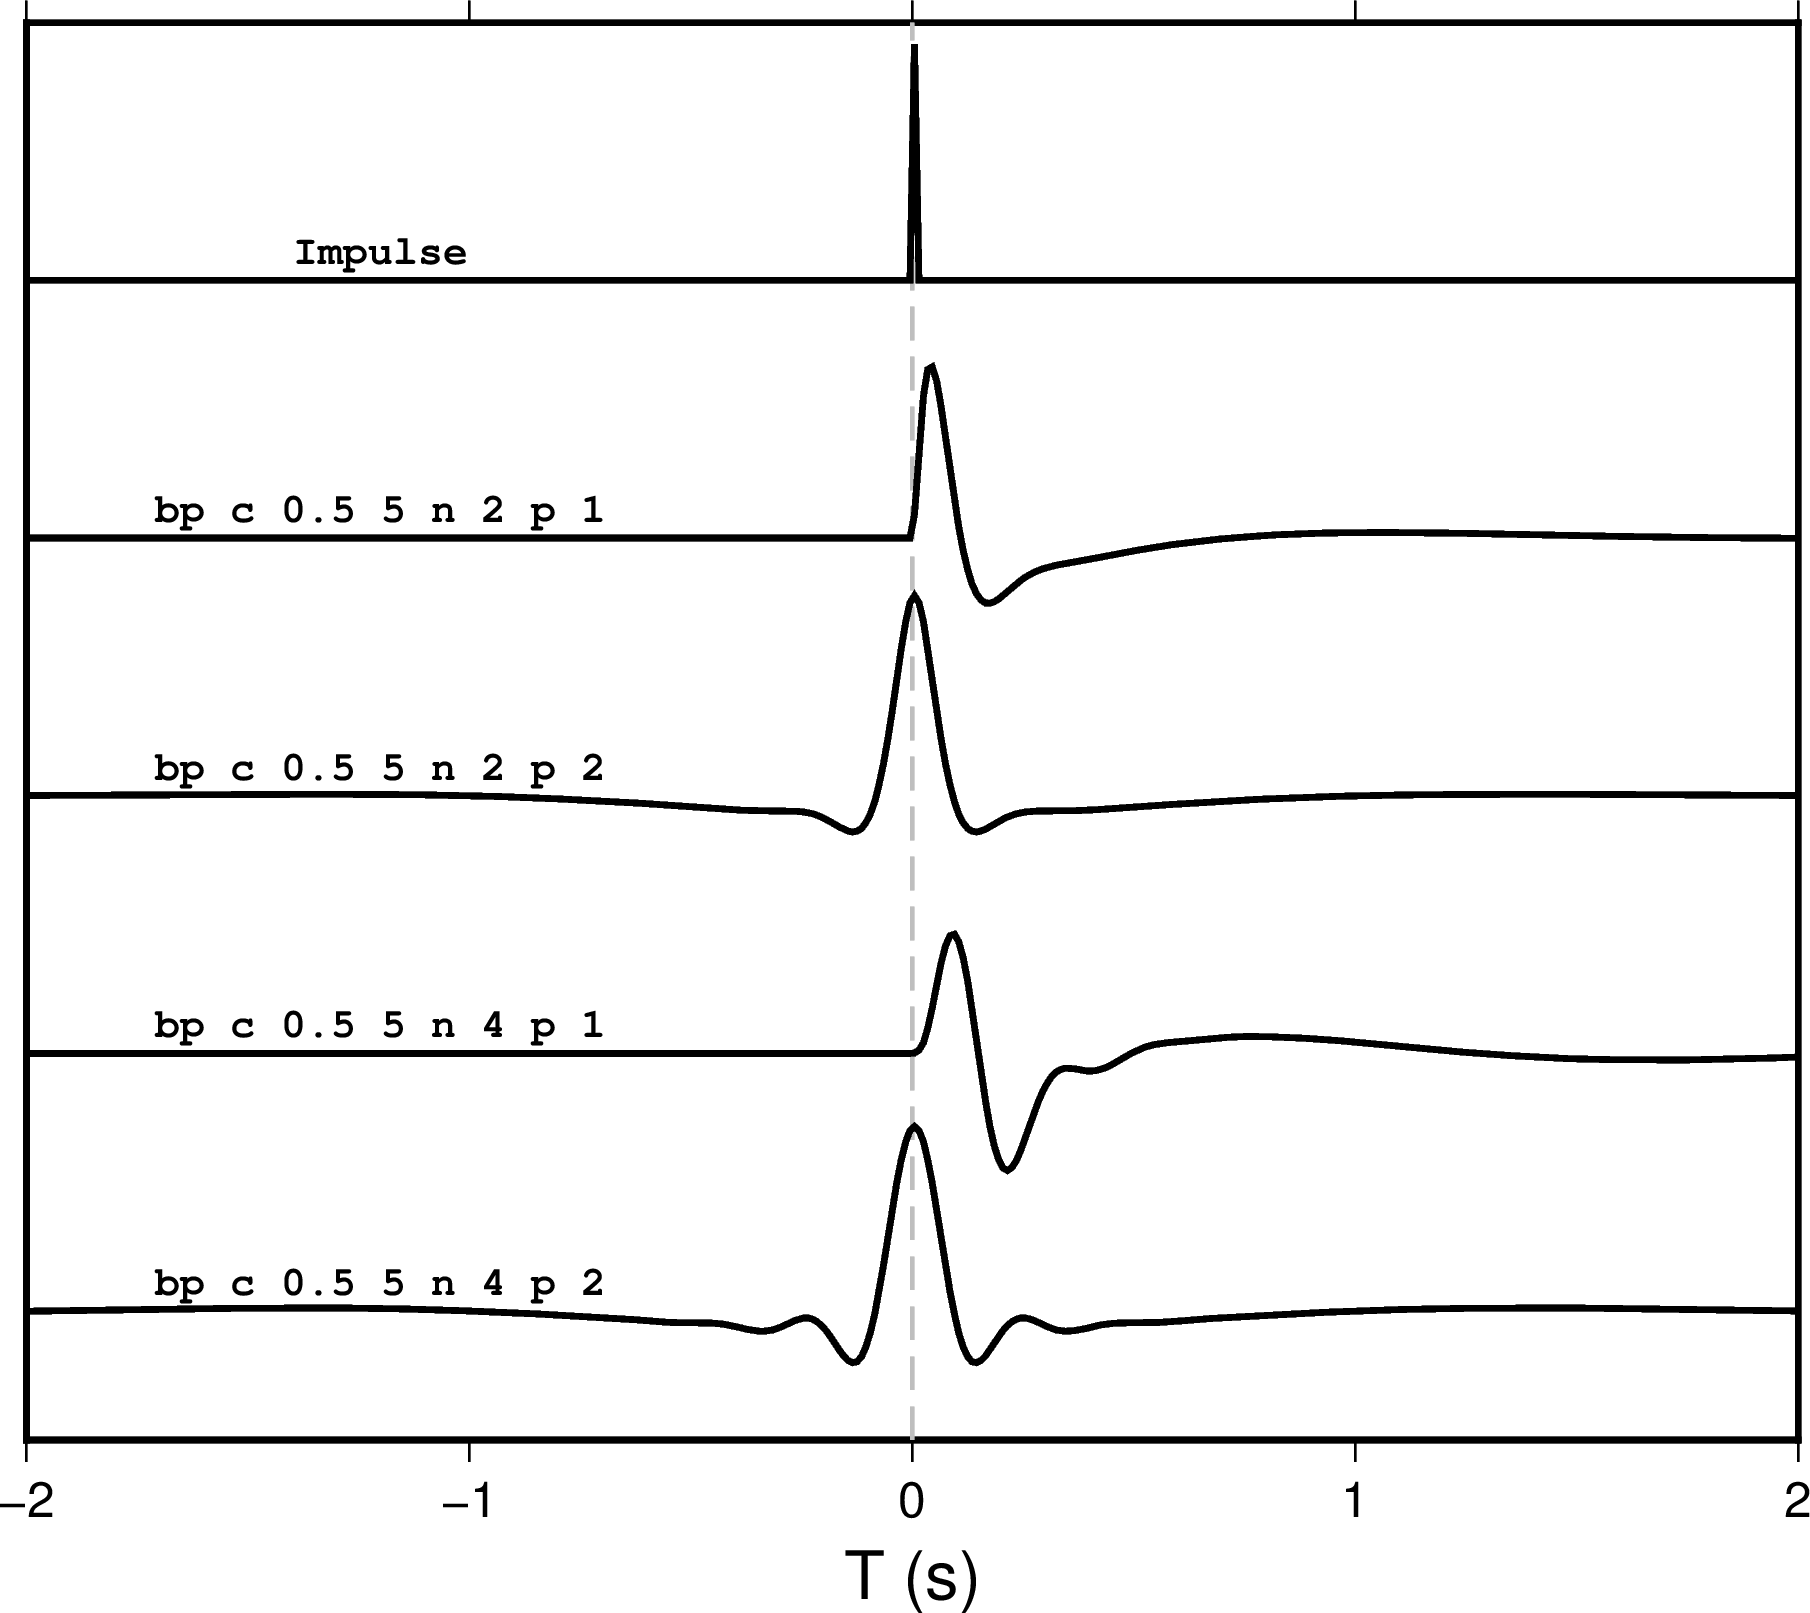
\includegraphics[width=0.8\textwidth]{filter-waveform}
\caption{不同参数的带通滤波效果}
\label{fig:filter-waveform}
\end{figure}
图 \ref{fig:filter-waveform} 中Impulse为原始脉冲波形,下面四条波形是分别取不同的n
值和p值的结果。

p取1时,对波形做一次带通滤波,由于滤波器存在相位延迟,因而导致波形的峰值出现了时间
延迟,因而会影响到震相的最大峰值的拾取,但对震相的初至却没有影响。

p取2时,对波形做正反两次带通滤波,此时不存在相位延迟,因而不会影响到最大峰值的拾取,
但震相的初至则存在时间上的提前。
